\chapter{Methodology \& Implementation}

\renewcommand{\chaptername}{Chapter}
\section*{Introduction}

This chapter details the methodology and implementation of the proposed path planning system for logistics forklifts, 
focusing on guiding the robot to a pallet in the tight spaces of a warehouse. The system uses pattern-based paths with 
splines, optimized by meta-heuristic algorithms, to navigate efficiently in these confined areas. The chapter begins with 
an overview of the design structure, followed by a clear explanation of the steps and techniques used to ensure 
smooth and accurate movement toward the pallet. Implementation details are then covered, showing how the system 
components are integrated into a cohesive solution for precise pallet access within the warehouse environment.

\section{Methodology }
%goals and overall approach of the methodology
Considered the problems detailed in chapter 1, the following goals were identified based on the company's vision and the 
general requirements for applications to autonomous mobile robots in intralogistics:
\begin{itemize}
    \item \textbf{Predictability and Robustness of Mobile Robot Behavior: }The solution utilizes an intelligent approach to connect 
    the robot to its destination. The developed algorithm generates an explainable navigation process that enables humans 
    to understand and trust the technology. Additionally, secure decision-making for autonomous trucks is ensured by the 
    developers. 

    \item \textbf{Accuracy of the solution and station relation: }The developed solution is stable, repeatable and flexible: this 
    means that it would work for almost all stations in warehouses where it operates. The linking to the destination is 
    accurate and precise to avoid failures. Precision and accuracy are guaranteed by the fact that the planning is done 
    in the limited station space: a narrow field that allows short distance perception and planning. The solution is 
    then tailored to each environment's specificities. 
    
    \item \textbf{Optimization of paths: }The algorithm optimizes the path by minimizing travel distance, reducing sudden turns, and avoiding challenging maneuvers that could 
    strain the truck. This optimization ensures the most efficient route, balancing speed and safety. The approach is designed to be 
    computationally efficient, allowing for real-time adjustments and smooth behavior of the autonomous truck.

    \item \textbf{Obstacle avoidance: }The vehicle avoids collisions and drives safely to its destination. The system is designed to 
    prioritize safety while maintaining an efficient and effective route to the target location.

\end{itemize}

Starting with the operating environment, the stations, the focus was on the problems inside. The issue of linking 
the forklifts in the near-field to the pallet is nothing but new to the intralogistics sector. 
The process is repeated dozens of times daily inside warehouses and factories where forklift drivers take control over 
resolving the problem. Taking a deeper look at their approaches to resolve the same issue, the autonomous vehicles team 
noticed that forklift drivers have certain driving styles that are repeated according to the current situation.
Similarily to car parking, depending on the type of the parking slot, there are some patterns to reproduce in order to fit 
the car inside its assigned spot as given by figure \ref{Parking Styles}. In case of a backward parking, the driver needs 
enough space for direction changing. To do so, he drives further to the opposite direction to allow 
the car to comfortably and smoothly drive to its parking place.
Parking assistance feature is embedded in human-driven and driverless cars to instill safety and order.

Analogically, after the truck arrives in the station, the drivers would drive and steer in the opposite direction of the 
pallet, until the forks are in a position to allow the truck to easily and correctfully drive to the pallet in fork direction.
The goal here is to develop a pallet-linking assistance algorithm to facilitate the driving and pallet pickup process for 
autonomous forklifts as given by figure \ref{pattern}. The truck would autonomously plan the path to its destination
based on the pattern and on the environment settings that it would navigate in. 
%TODO: explain predictability

\begin{figure}
    [H]
    \begin{center}
    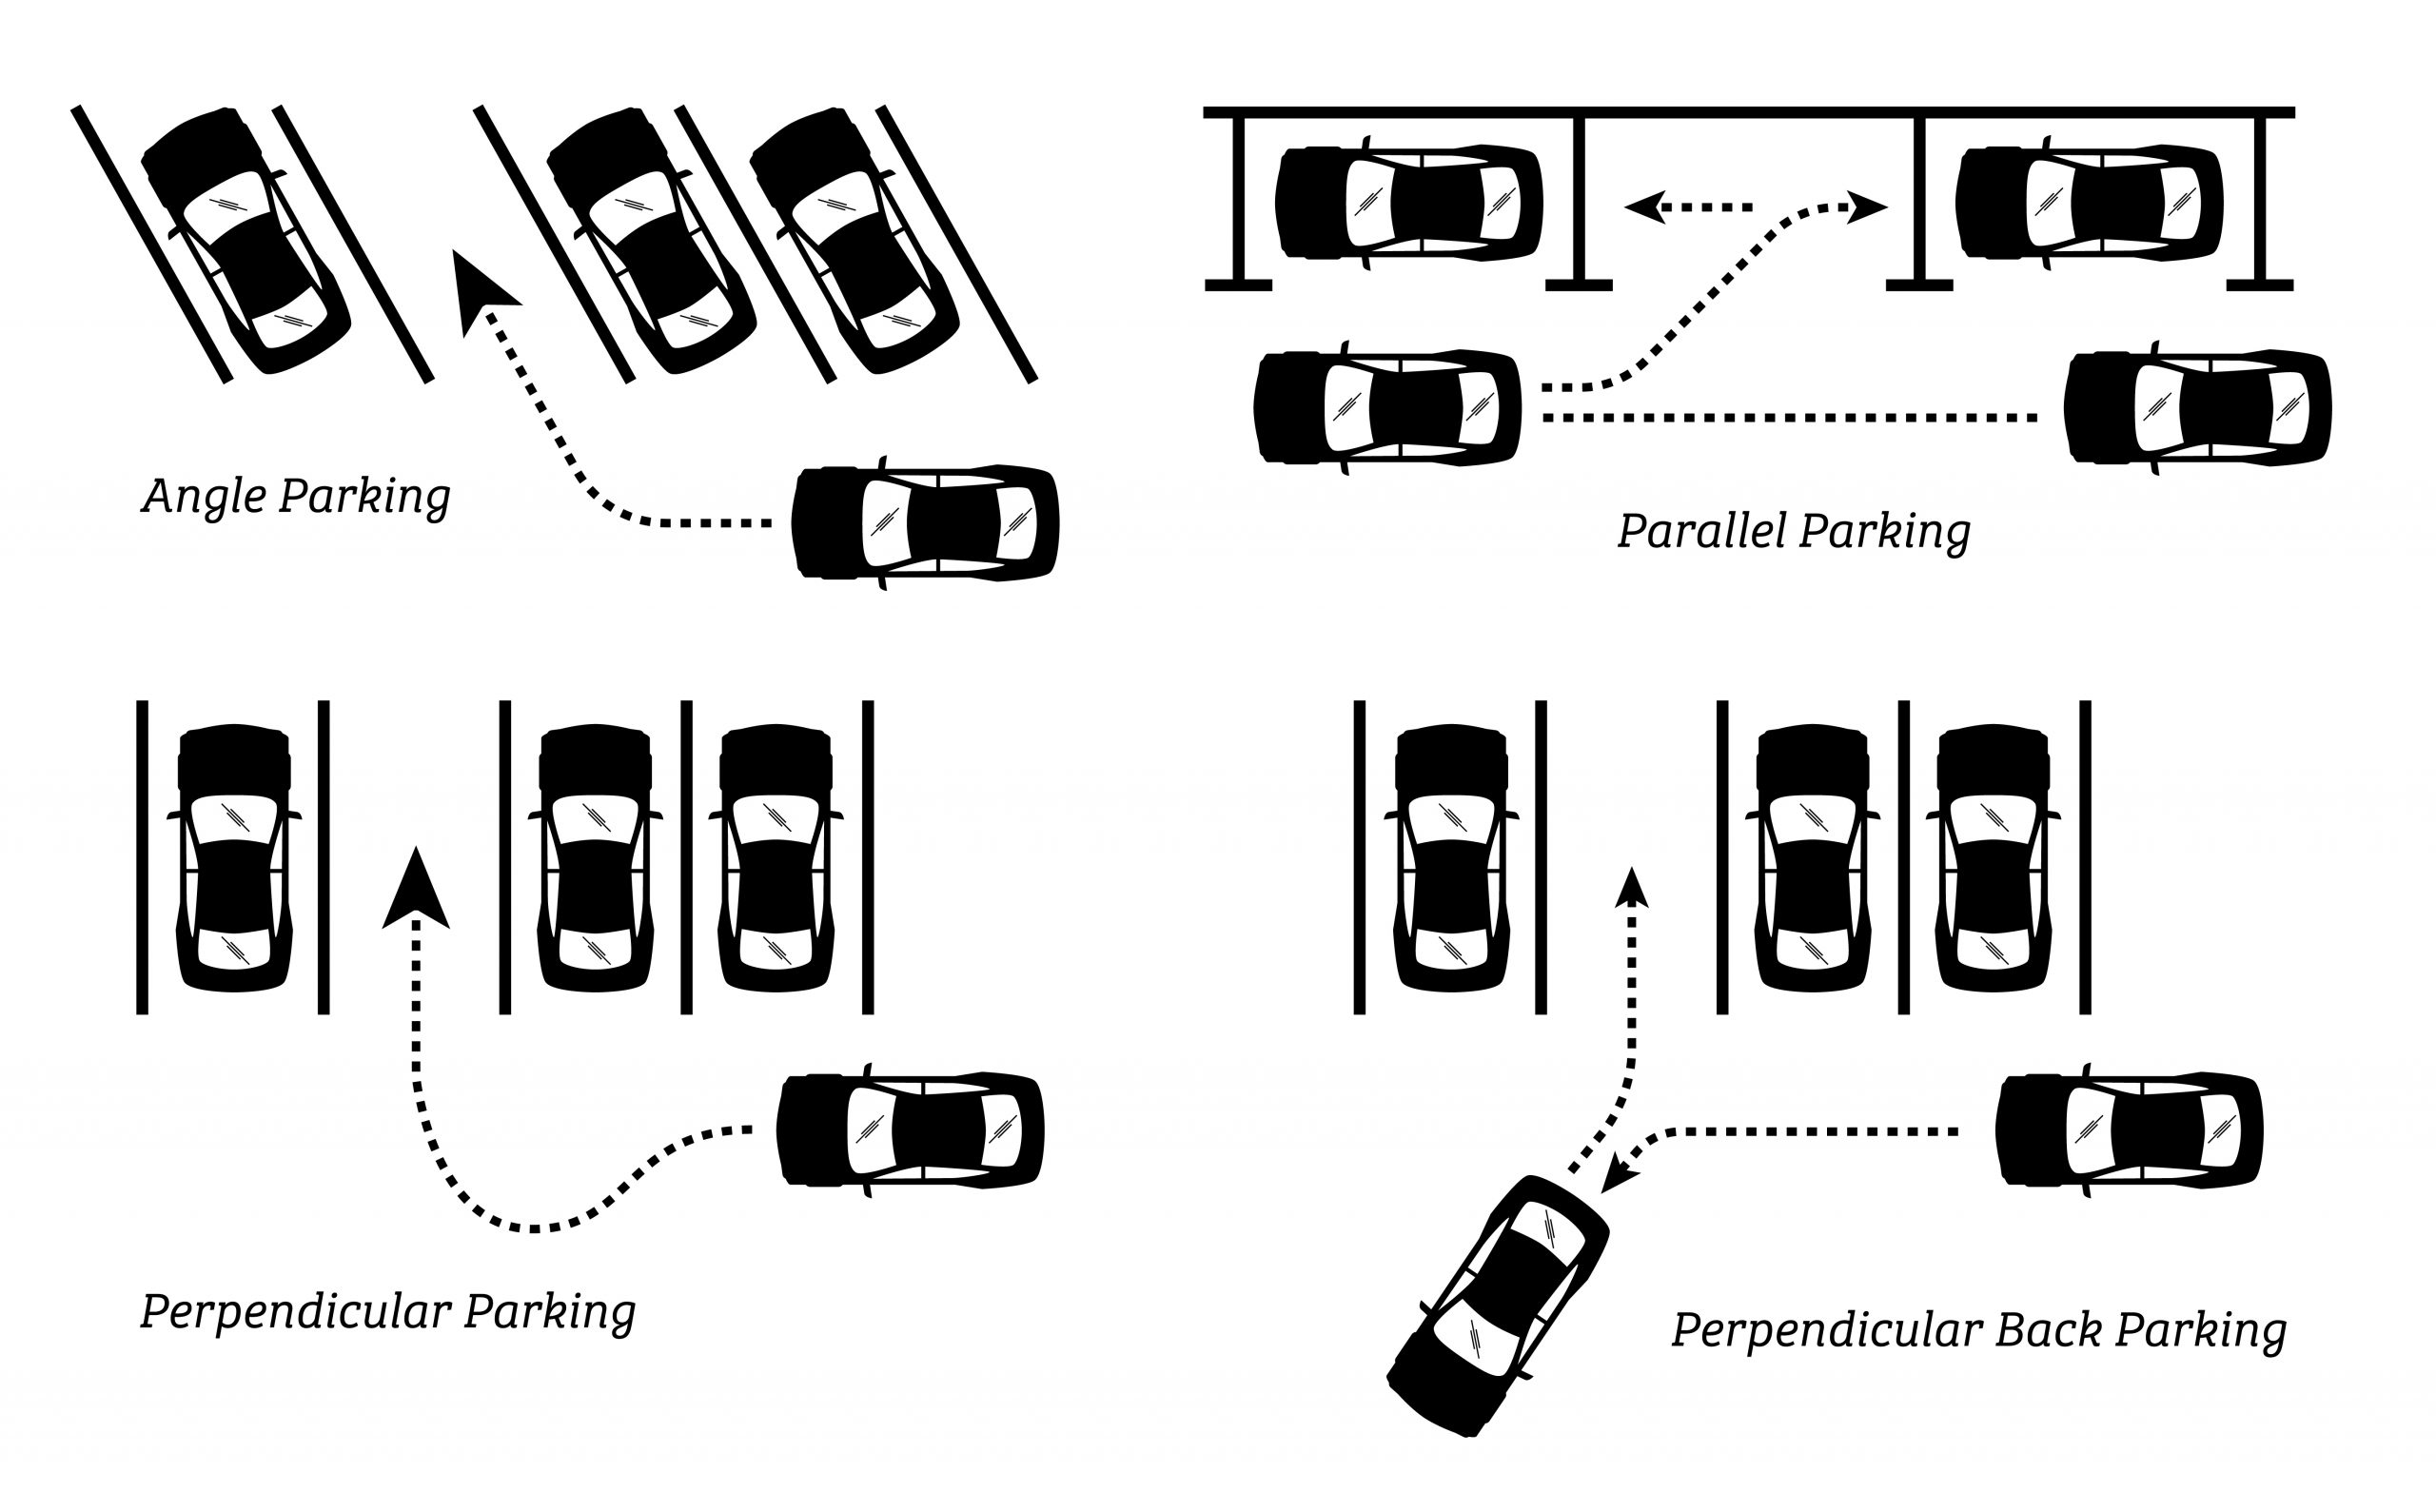
\includegraphics[width=4in]{images/Chap2/perpendicular-parking-a-lot-scaled.jpg}\\
    \caption{Parking Styles}
    \label{Parking Styles}
    \end{center}
\end{figure}


\begin{figure}
    [H]
    \begin{center}
    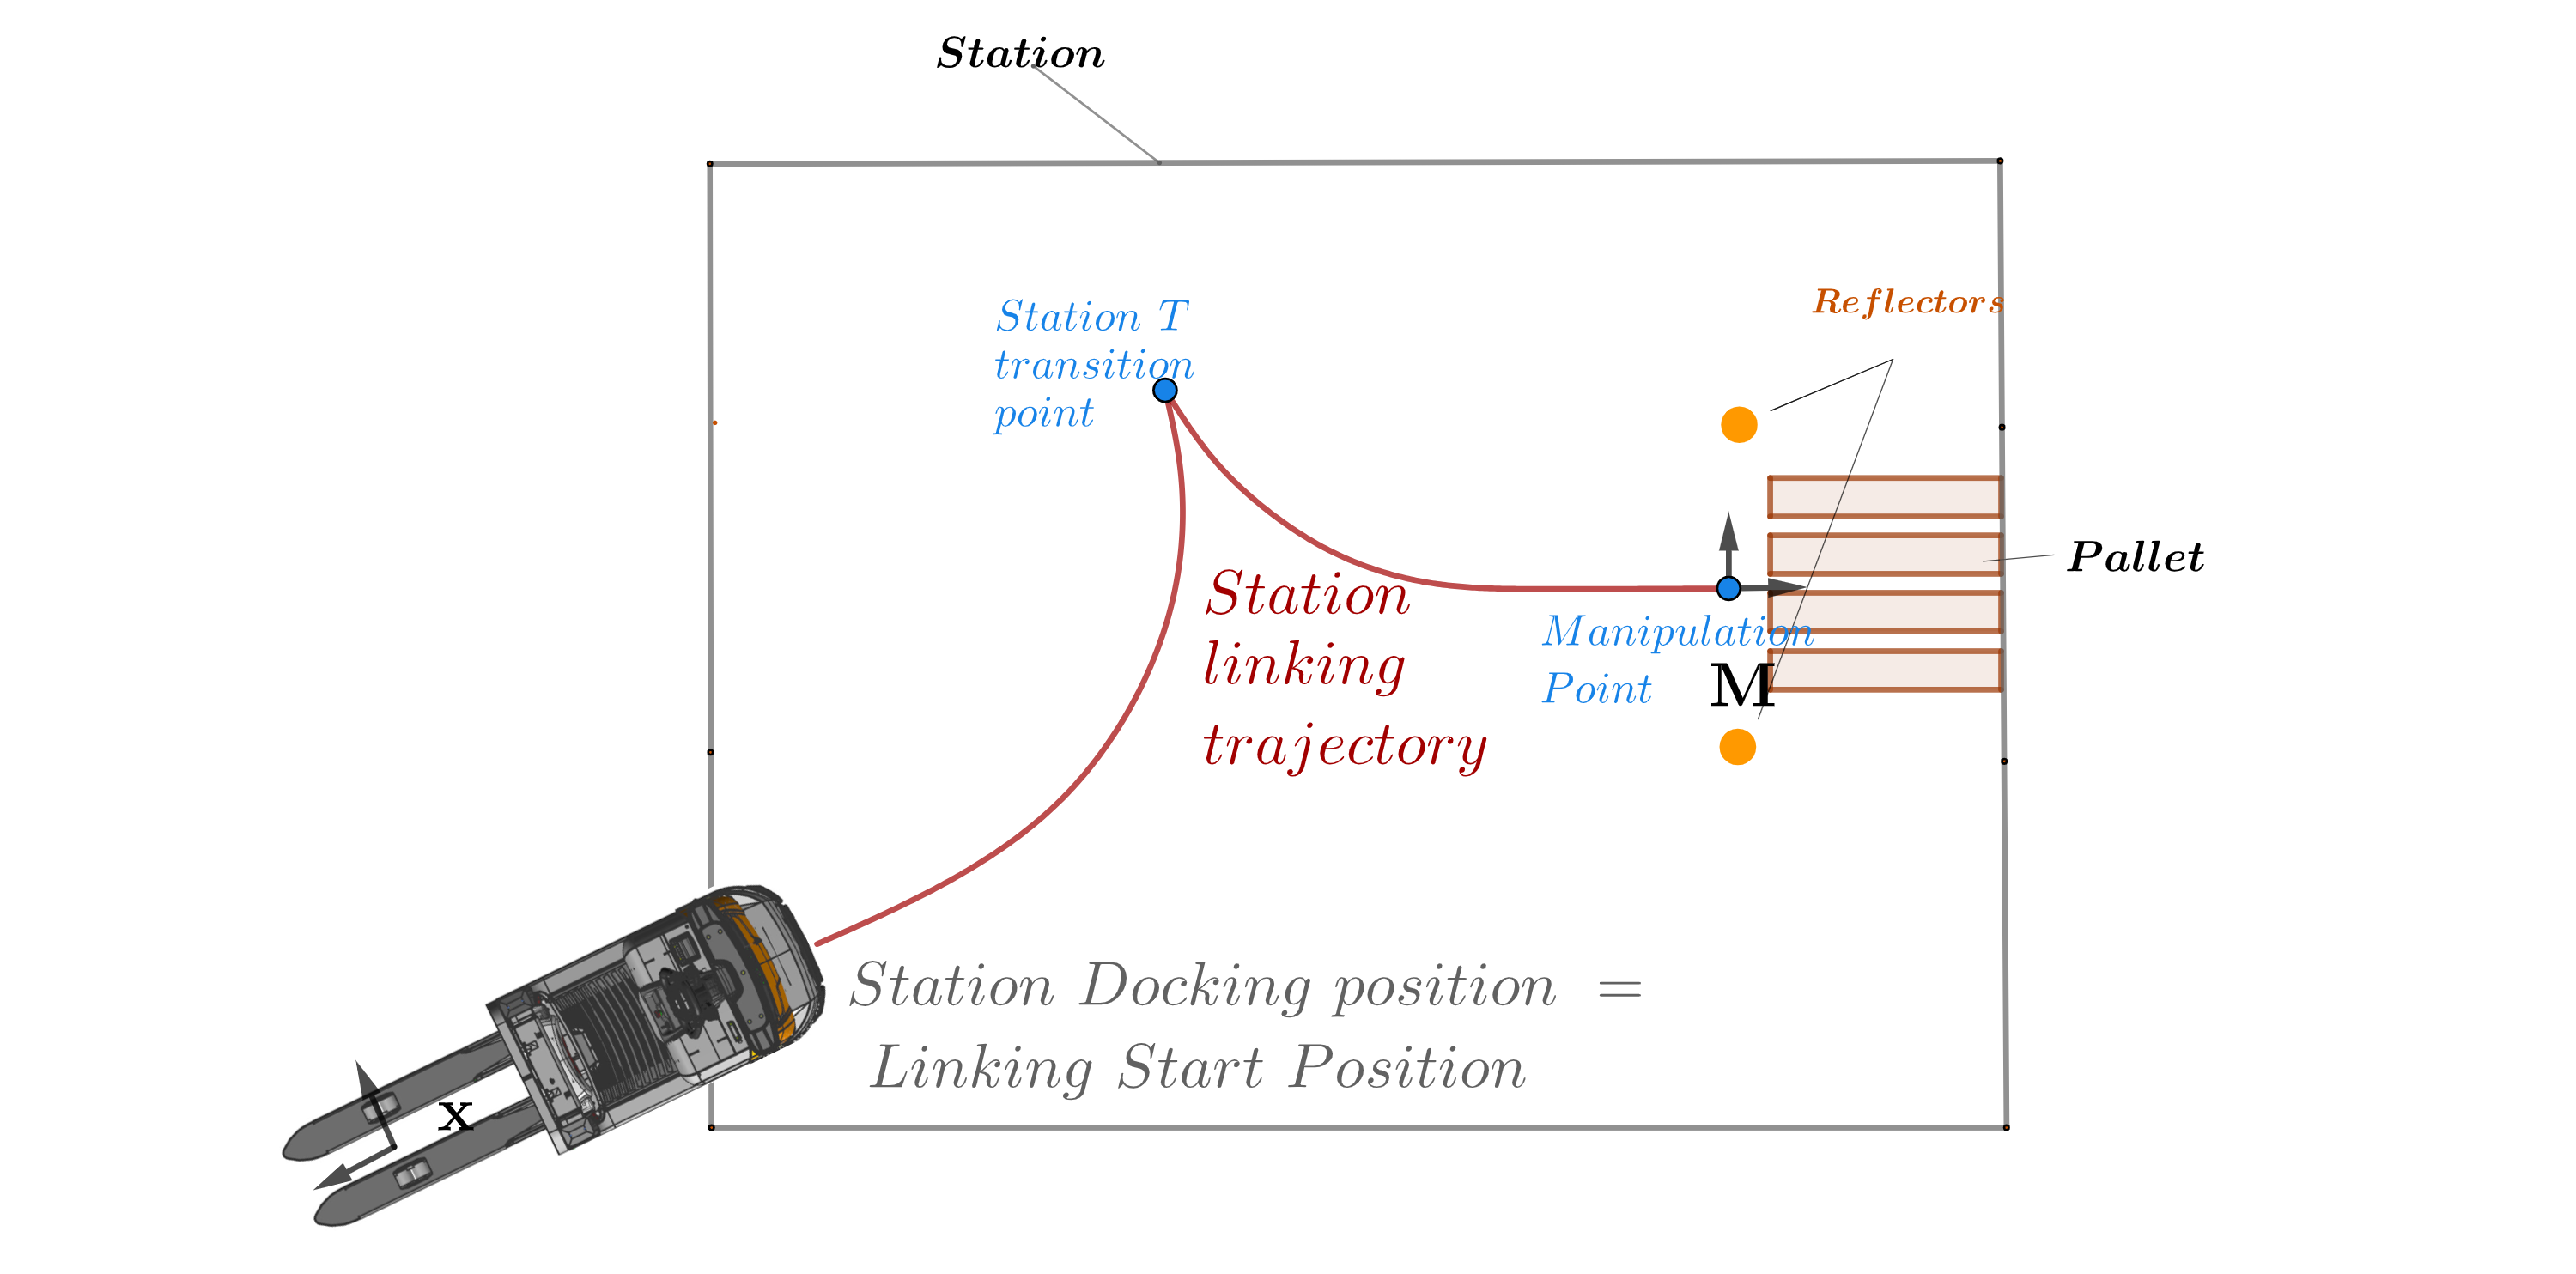
\includegraphics[width=\linewidth]{images/Chap2/station-without-subpolygones.png}\\
    \caption{Linking the robot to goal destination \cite{R28}}
    \label{pattern}
    \end{center}
\end{figure}
From now on, the following definitions of driving directions will be used as gven by figure \ref{driving directions}:
\begin{itemize}
    \item Main Driving Direction: Driving in fork direction.
    \item Opposite Driving Direction: Driving in vehicle chassis direction.
\end{itemize}

\begin{figure}
    [H]
    \begin{center}
    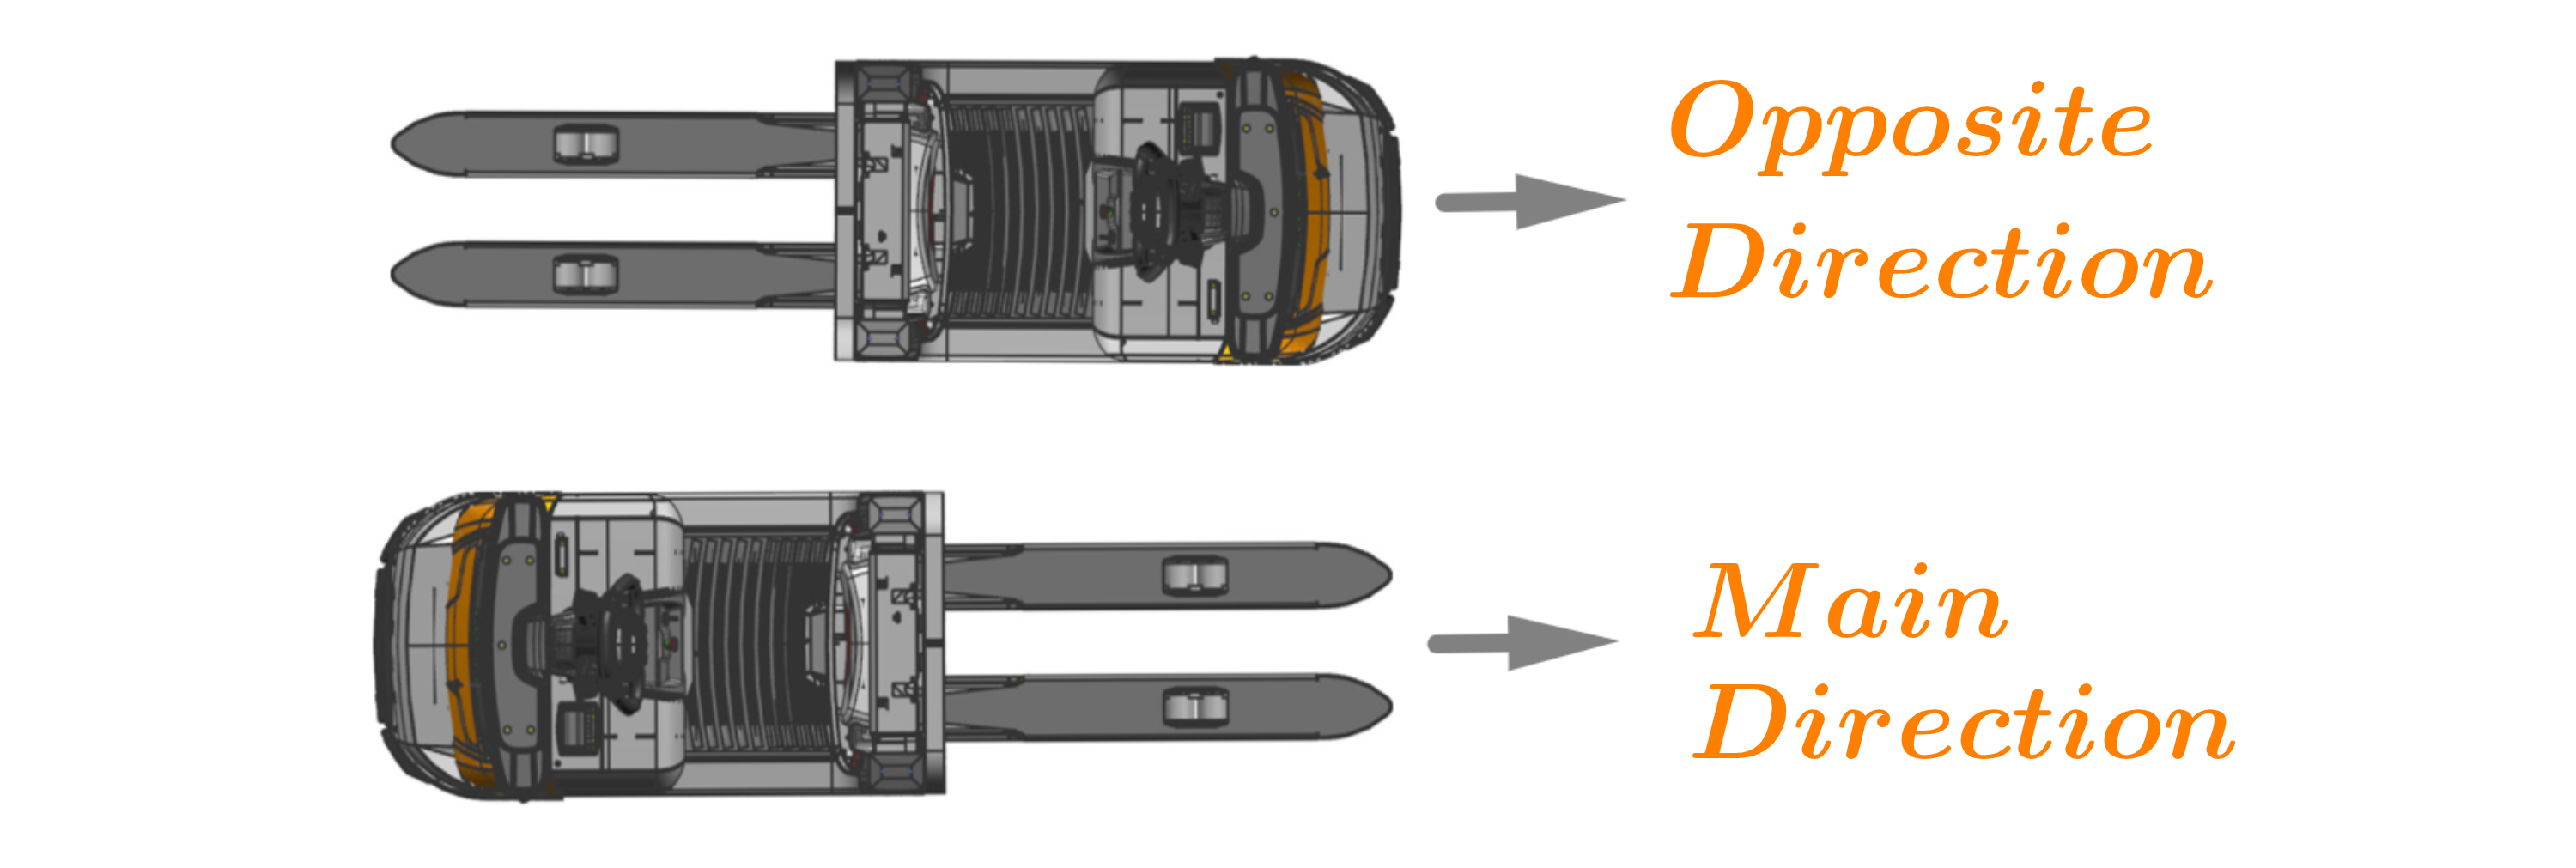
\includegraphics[width=4in]{images/Chap2/driving_directions.png}\\
    \caption{Truck Driving Directions}
    \label{driving directions}
    \end{center}
\end{figure} 
 
The following transition method is suggested: once the truck docks the station, it has the option to transition and change 
direction on the sides of the station. First, it drives to the transition position, then, to the pallet or the drop-off position
as given by figure \Ref{subpolygones}. Having two possibilities for transition zones allows for more flexibility

\begin{figure}
    [H]
    \begin{center}
    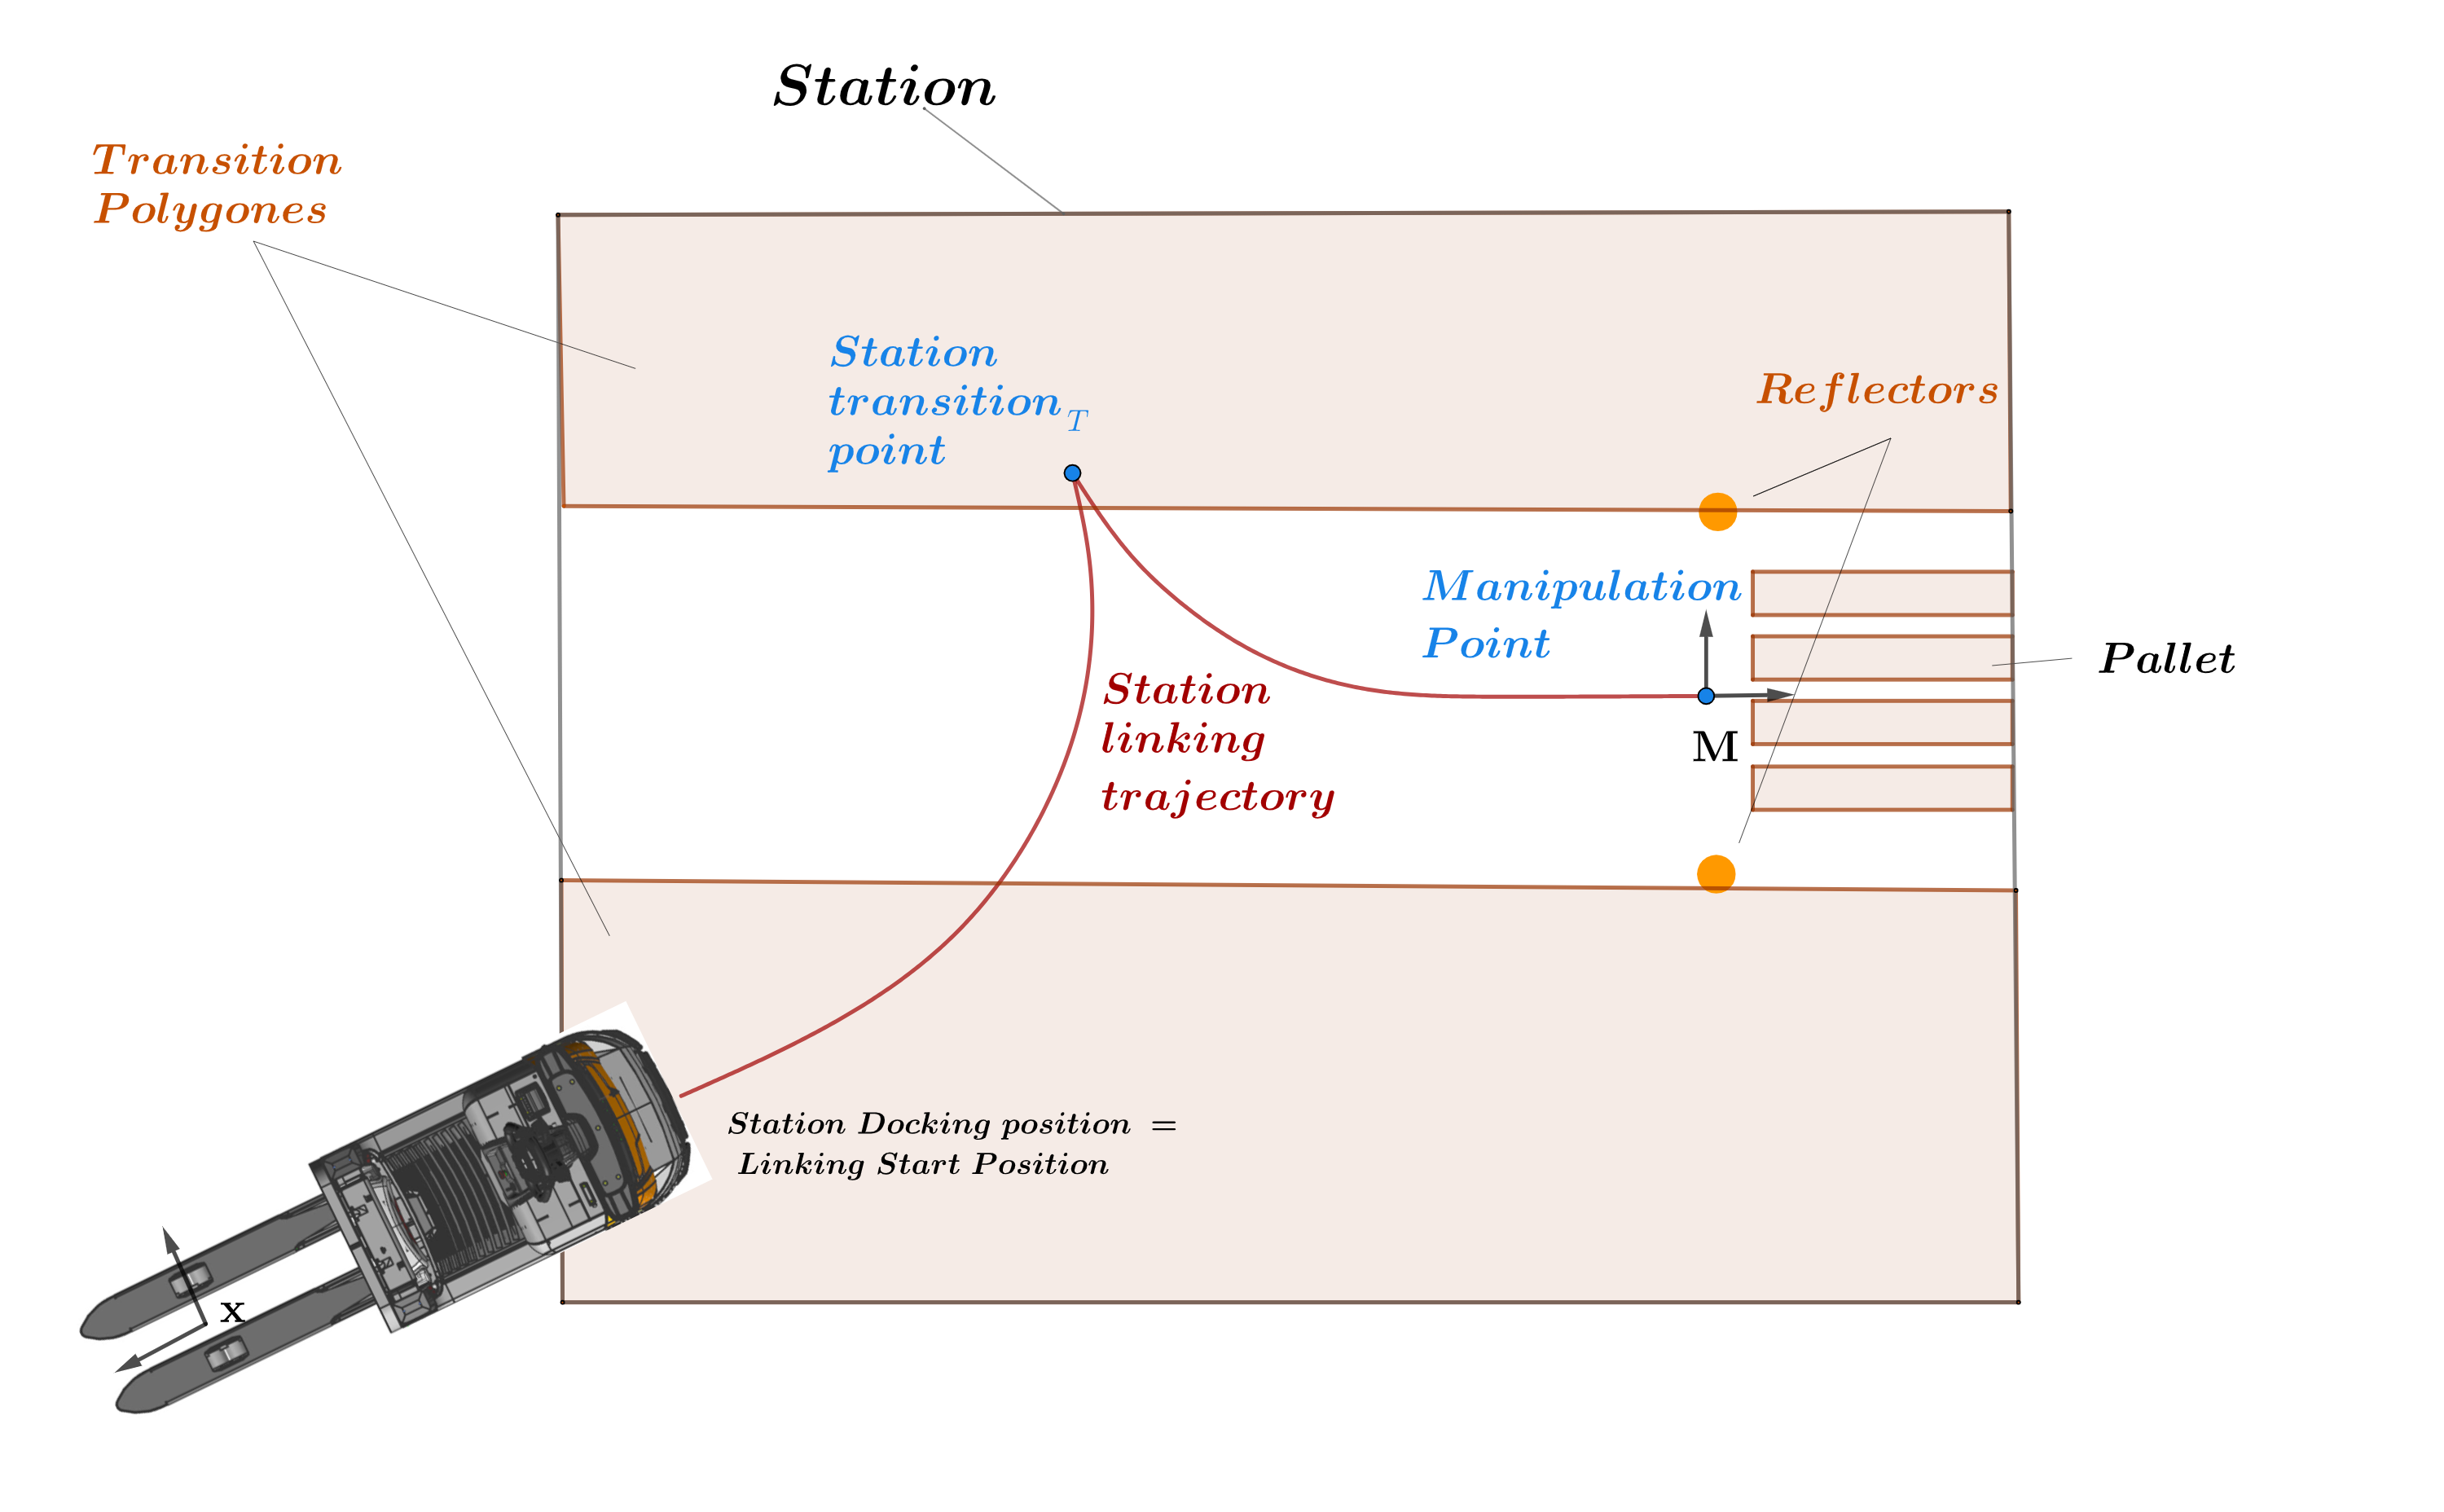
\includegraphics[width=\linewidth]{images/Chap2/station-without-subpolygones (2).png}\\
    \caption{Linking the robot to goal pallet \cite{R28}}
    \label{subpolygones}
    \end{center}
\end{figure}


